\documentclass{article}
\usepackage{amsmath}
% \usepackage{cancel}
\usepackage{fancyhdr}
\usepackage{graphicx}

% \pagestyle{fancy}
% \fancyfoot{}
% \lfoot{\copyright\ Christopher A. Bohn}
% %% (c) 2018-22
% \rfoot{Page \thepage}

\fancypagestyle{plain}{
    \fancyhf{}
    \lfoot{\copyright\ Christopher A. Bohn} % (c) 2018-22
    \rfoot{Page \thepage}
    \renewcommand{\headrulewidth}{0pt}
    \renewcommand{\footrulewidth}{0pt}
}
\pagestyle{plain}

\newcommand{\carry}{\scriptstyle 1}

\begin{document}

\title{Chapter 4 Worked Examples}
\date{}
\maketitle

\section{IEEE 754 Format}

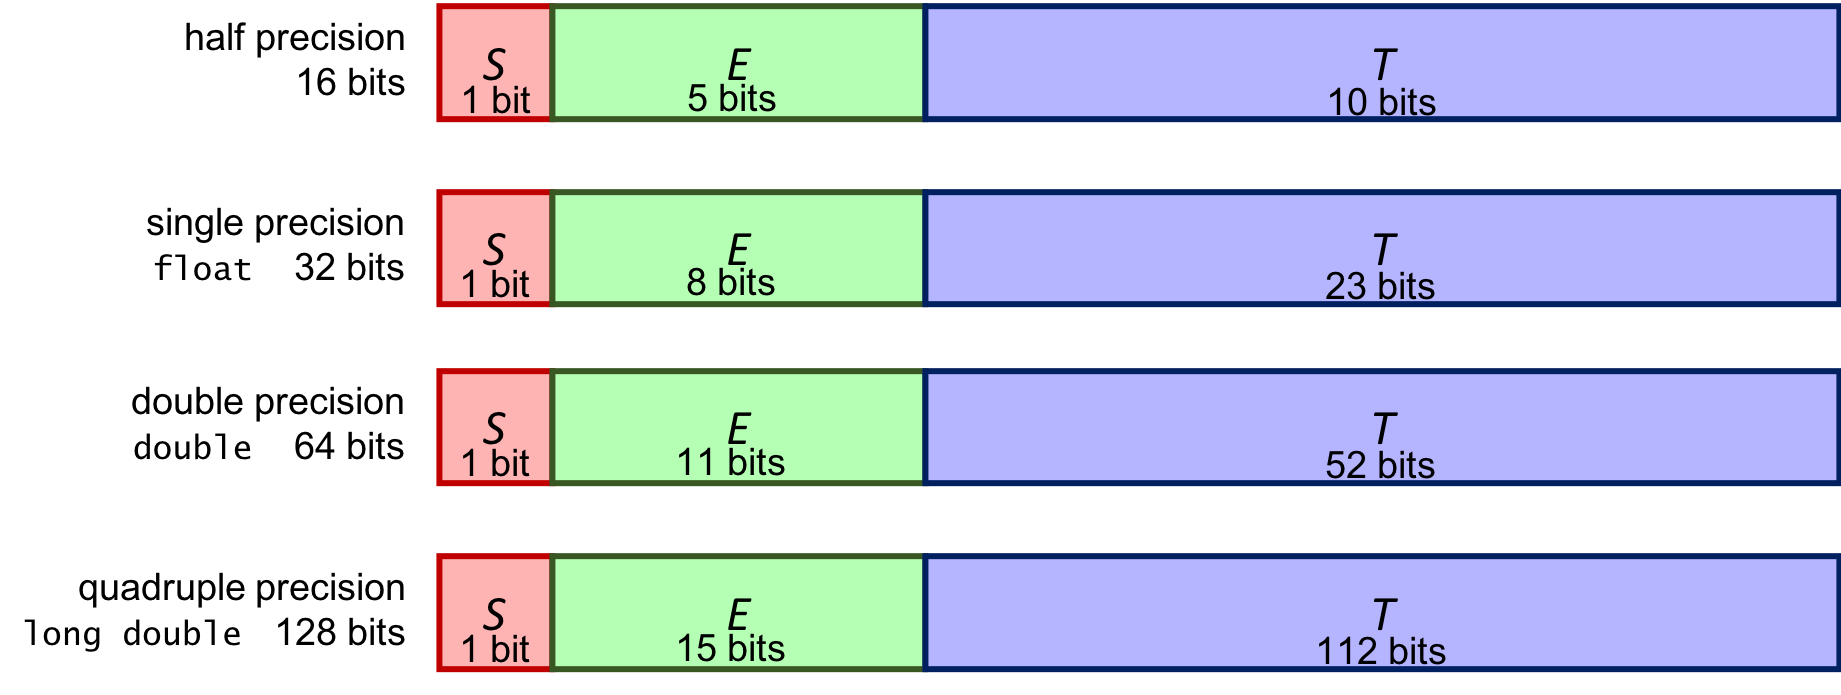
\includegraphics[width=\textwidth]{754-precisions.png}

\vspace{1cm}

Verbally, we'll refer to the \textit{T} field as the \textit{fraction} field.

\begin{itemize}
\item Sign bit is 0 for positive, 1 for negative
\item \textit{E} field encodes the exponent as a \textbf{biased integer}
    \begin{itemize}
    \item $bias = 2^{w-1} - 1$, where $w$ is the width of the \textit{E} field
    \end{itemize}
\item \textit{T} field holds the fraction -- we can encode the significand by
    storing only the fraction because the integer portion of the significand is
    guaranteed to be 1 (normal numbers) or 0 (subnormal numbers)
\end{itemize}

\subsection{Normal Numbers}

\begin{itemize}
\item $00\dots01 \leq E \leq 11\dots10$
\item $exponent = E - bias$
\item $m = 1.T$ or $m = 1.fraction$
\end{itemize}

\subsection{Subnormal Numbers}

\begin{itemize}
\item $E = 00\dots00$
\item $T \neq 00\dots00$
\item $exponent = 1 - bias$
\item $m = 0.T$ or $m = 0.fraction$
\end{itemize}

\subsection{$\pm$Zero}

\begin{itemize}
\item $E = 00\dots00$
\item $T = 00\dots00$
\item Technically not a subnormal number; this is mostly a distinction without a
    difference, except\dots
\item +0 = -0
\end{itemize}

\subsection{$\pm$Infinity}

\begin{itemize}
\item $E = 11\dots11$
\item $T = 00\dots00$
\end{itemize}

\subsection{Not-a-Number (NaN)}

\begin{itemize}
\item $E = 11\dots11$
\item $T \neq 00\dots00$
\end{itemize}


\section{Quarter-Precision Floating Point}

Not a real IEEE 754 precision, but useful for classroom use

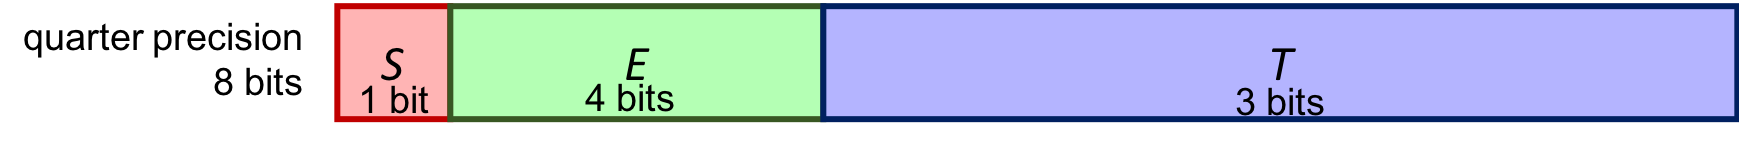
\includegraphics[width=\textwidth]{quarter-precision.png}

\section{Converting Between Mixed Fractions and Exact Fixed Point Binary Numbers}

\[7\frac{5}{16}\]

\begin{itemize}
\item The integer portion is expressed (in binary) to the left of the binary
    point (here, 111)
\item The exact value will require $\log_2{denominator}$ bits to the right of
    the binary point (here, 4 bits)
\item Use those bits to the right of the denominator to express the numerator
    (here, 0101)
\end{itemize}

\[111.0101_{2}\]

Conceptually, $7\frac{5}{16}$ in decimal is $111\frac{101}{10000}$ in binary,
and now you should be able to see that it's pretty much the same as converting
a mixed fraction (with a denominator that's a power of 10) to decimal fixed
point.

Going the other direction

\begin{itemize}
\item The integer portion is the part that's to the left of the binary point
    (here, $111_2 = 7_{10}$)
\item If the portion to the right of the binary point uses $n$ bits, then the
    denominator is $2^n$ (here, $2^4=16$)
\item The numerator is the actual value to the right of the binary point (here,
    $0101_2=5_{10}$)
\end{itemize}

\section{Half-Precision Floating Point Non-Rounding Examples}

\begin{itemize}
\item 1 bit for the sign
\item 5 bits for the \textit{E} field
    \begin{itemize}
    \item $bias = 2^{5-1} - 15$
    \end{itemize}
\item 10 bits for the fraction
\end{itemize}

\subsection{Going to IEEE 754 format}

(note we're including spacing in the fraction for readability)

\begin{align*}
9\frac{35}{128} &= 1001.0100\ 011_2 \\
                &= 1.0010\ 1000\ 11_2 \times 2^{3}
\end{align*}

\begin{itemize}
\item Positive $\Rightarrow S=0$
\item $E = 3_{10} + 15_{10} = 18_{10} = 10010$
\item $fraction = 0010100011$
\end{itemize}

Combining those, we get $0\ 10010\ 0010100011$, or 0x48A3 (here, we're simply
expressing the bit pattern in hex as shorthand; we are not saying that
$9\frac{35}{128} = 18,595_{10}$).

\vspace{1.5cm}

\begin{align*}
-\frac{792}{2048}   &= -0.0110\ 0011\ 000_2 \\
                    &= -1.1000\ 1100\ 0_2 \times 2^{-2}
\end{align*}

\begin{itemize}
\item Negative $\Rightarrow S=1$
\item $E = -2_{10} + 15_{10} = 13_{10} = 01101$
\item $fraction = 1000110000$ (notice that we added an extra 0 on the right to
    fill it out to 10 fractional bits)
\end{itemize}

Combining those, we get $1\ 01101\ 1000110000$, or 0xB630.

\vspace{1.5cm}

\begin{align*}
-1234   &= -100\ 1101\ 0010._2 \\
        &= -1.0011\ 0100\ 10_2 \times 2^{10}
\end{align*}

\begin{itemize}
\item Negative $\Rightarrow S=1$
\item $E = 10_{10} + 15_{10} = 25_{10} = 11001$
\item $fraction = 0011010010$
\end{itemize}

Combining those, we get $1\ 11001\ 0011010010$, or 0xE4D2.

\subsection{Coming from IEEE 754 format}

\[\mathrm{94CA} = 1001\ 0100\ 1100\ 1010 = 1\ 00101\ 0011001010\]
(adjusted spacing to clearly identify the bit fields)

\begin{itemize}
\item $S=1 \Rightarrow$ Negative
\item $E = 00101 = 5_{10} \Rightarrow exponent = 5-15 = -10$
\item $fraction = 0011001010 \Rightarrow m = 1.0011001010$
\end{itemize}

\[1.0011001010_2 \times 2^{-10} = 0.0000\ 0000\ 0100\ 1100\ 1010_2 = -\frac{1226}{2^{20}}= -\frac{1226}{1,048,576}\]

\vspace{1.5cm}

\[\mathrm{0x6D39} = 0110\ 1101\ 0011\ 1001 = 0\ 11011\ 0100111001\]

\begin{itemize}
\item $S=0 \Rightarrow$ Positive
\item $E = 11011 = 27_{10} \Rightarrow exponent = 27-15 = 12$
\item $fraction = 0100111001 \Rightarrow m = 1.0100111001$
\end{itemize}

\[1.0100111001_2 \times 2^{12} = 1 0100 1110 0100._2 = 5,348\]

\vspace{1.5cm}

\[\mathrm{0x5F27} = 0101\ 1111\ 0010\ 0111 = 0\ 10111\ 1100100111\]

\begin{itemize}
\item $S=0 \Rightarrow$ Positive
\item $E = 10111 = 23_{10} \Rightarrow exponent = 23-15 = 8$
\item $fraction = 1100100111 \Rightarrow m = 1.1100100111$
\end{itemize}

\[1.1100100111_2 \times 2^{8} = 111001001.11_2 = 457\frac{3}{4}\]

\subsection{Subnormal Examples}

\[\mathrm{0x819B} = 1000\ 0001\ 1001\ 1011 = 1\ 00000\ 0110011011\]

\begin{itemize}
\item $S=1 \Rightarrow$ Negative
\item $E = 00000 \Rightarrow$ subnormal $\Rightarrow exponent = 1 - bias = 1 - 15 = -14$
\item $fraction = 0110011011\ and\ \mathrm{subnormal} \Rightarrow m = 0.0110011011$
\end{itemize}

\[-00110011011_2 \times 2^{-14} = -0.0000\ 0000\ 0000\ 0001\ 1001\ 1011_2 = -\frac{411}{2^{24}} = -\frac{411}{16,777,216}\]

\vspace{1.5cm}

\begin{align*}
\frac{32}{2^{26}}   &= 0.0000\ 0000\ 0000\ 0000\ 0000\ 1100\ 00_2 \\
                    &= 1.10000_2 \times 2^{-21}
\end{align*}

Since the bias is 15 (and so $exponent + bias = -6$), this is clearly too small
for the normal form. Let's re-express it with $exponent=-14$ (because
$-14 = 1 - bias$).

\[1.10000_2 \times 2^{-21} = 0.0000\ 0011\ 0000_2 \times 2^{-14}\]

Even if you know nothing about rounding, I think you can agree that can be
``rounded'' to

\[0.0000\ 0011\ 00_2 \times 2^{-14}\]

\begin{itemize}
\item Positive $\Rightarrow S=0$
\item subnormal $E = 00000$
\item $fraction = 0000001100$
\end{itemize}

Combining those, we get $0\ 00000\ 0000001100$, or 0x000C.

\section{Quarter-Precision Floating Point Rounding Examples}

We aren't going to encode these in the pseudo-754 8-bit format; we're simply
going to limit ourselves to 3 bits in the fraction.

\begin{itemize}
\item Look at bits that will get rounded-off
    \begin{itemize}
    \item MSB of rounded-off portion is 0: round down (truncate)
    \item MSB of rounded-off portion is 1 and there is at least one other 1 in
        the rounded-off portion: round up (add 1 to the LSB of the portion that
        doesn't get rounded-off)
    \item MSB of rounded-off portion is 1 and there are no other 1s in the
        rounded-off portion: round to nearest-even (round up or down to make
        the remaining LSB a 0)
    \end{itemize}
\item Renormalize if necessary
\end{itemize}

\begin{align*}
1.011\ 01001 \times 2^5     & \rightarrow 1.011 \times 2^5 \\
1.110\ 00011 \times 2^{-3}  & \rightarrow 1.110 \times 2^{-3} \\
1.010\ 1001 \times 2^{-1}   & \rightarrow 1.011 \times 2^{-1} \\
1.101\ 111 \times 2^{2}     & \rightarrow 1.110 \times 2^2 \\
1.100\ 1000 \times 2^{0}    & \rightarrow 1.100 \times 2^{0} \\
1.001\ 10 \times 2^{-4}     & \rightarrow 1.010 \times 2^{-4} \\
1.111\ 1 \times 2^{3}       & \rightarrow 10.000 \times 2^{3} = 1.000 \times 2^{4} \\
1.111\ 11 \times 2^7        & \rightarrow 10.000 \times 2^7 = 1.000 \times 2^8 = \mathrm{Infinity}
\end{align*}

It also works for subnormal numbers:

\begin{align*}
0.010\ 0010 \times 2^{-6}   & \rightarrow 0.010 \times 2^{-6} \\
0.101\ 111 \times 2^{-6}    & \rightarrow 0.110 \times 2^{-6} \\
0.000\ 101 \times 2^{-6}    & \rightarrow 0.001 \times 2^{-6} \\
0.000\ 10 \times 2^{-6}     & \rightarrow 0.000 \times 2^{-6} = 0 \\
0.111\ 11 \times 2^{-6}     & \rightarrow 1.000 \times 2^{-6}\ \mathrm{which\ is\ now\ a\ normal\ number!}
\end{align*}

\end{document}
